\chapter{Introduction}

Zarafa provides an open source drop-in replacement for Microsoft Exchange Server, a messaging and groupware 
server product whose main features include e-mail, calendaring, and management of tasks and contacts. 
End users run a client application that connects to Exchange, most notably Microsoft Outlook or the web based
Outlook Web Access. Figure \ref{figure:stackms} shows the Microsoft messaging stack and how its products,
Exchange, Outlook, and Outlook Web Access relate to each other.

Zarafa offers alternatives to both Exchange Server and it's web access component. The Zarafa stack is 
shown in figure \ref{figure:stackzarafa}. End users of a Zarafa installation may either keep using 
Outlook (left) or choose to use the Zarafa Web Access (right). 

Evolution of browser technology, expressed in pervasiveness of new standards and improvements in
performance, have made it possible to build responsive and visually rich web applications with a 
'desktop' look and feel. Furthermore, open source libraries such as YUI and ExtJS significantly simplify
this task by providing a user interface framework with a rich set of standard components. 
Building on these new technologies, it is our ultimate ambition to build a web based alternative to 
not just Outlook Web Access, but also Outlook itself. 

This design document describes the architecture and implementation details of Zarafa's new web access.
Chapter \ref{section:ui} and \ref{section:communication} describe the user interface and communication 
protocols respectively. Chapter \ref{section:style} deals with code style and documentation practices.
Finally Chapter \ref{section:cookbook} contains detailed descriptions to show developers how to 
accomplish common tasks within our framework.

\begin{figure}[h!]
\centering
\subfigure[Microsoft]
{
	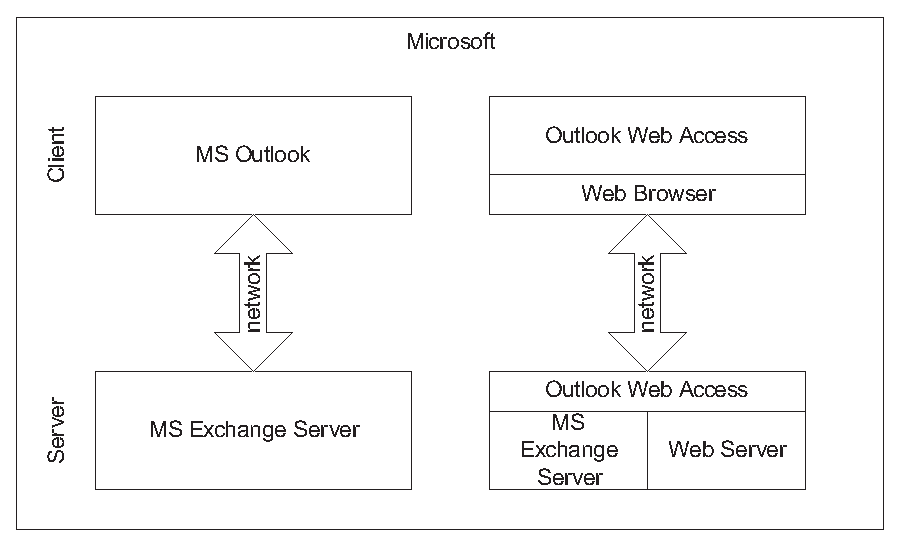
\includegraphics[width=7.5cm]{figures/stack_microsoft.eps}
	\label{figure:stackms}
}
\subfigure[Zarafa]
{
	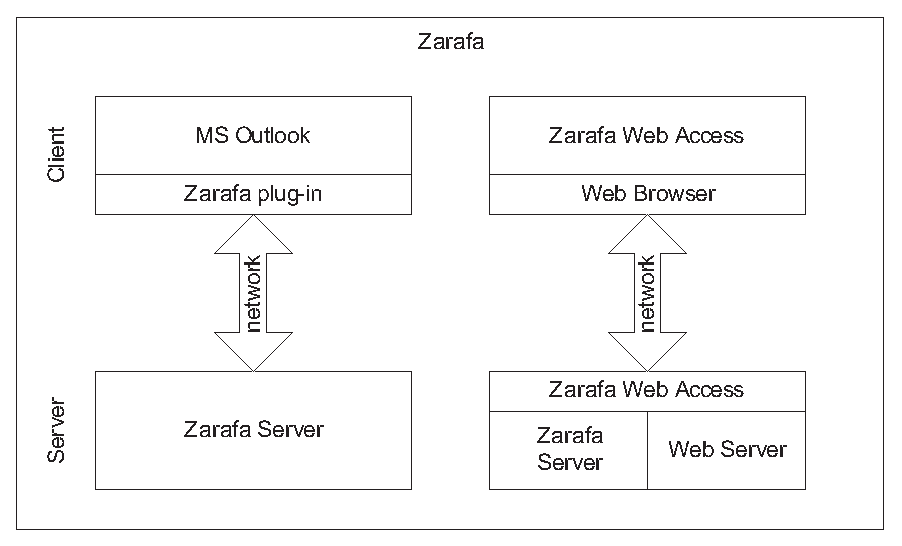
\includegraphics[width=7.5cm]{figures/stack_zarafa.eps}
	\label{figure:stackzarafa}
}
\caption{Comparison of messaging software stacks.}
\label{figure:mszarafacomparison}
\end{figure}
